\documentclass[bachelor,euler,twoside,openright]{ustcthesis}
% 默认twoside 双面打印
% 将master修改为bachelor, doctor or master
% 要使用adobe字体,添加adobefonts选项
% 要使用Mac系统的字体,添加macfonts选项
% 使用euler数学字体,如不愿使用,去掉euler
% 使用外文写作,请添加notchinese

% 设置图形文件的搜索路径
\graphicspath{{figures/}}

%仅用于本示例文档中显示特殊字符串
\usepackage{xltxtra}

%用于latex内作图

\usepackage{tikz,mathpazo}
\usetikzlibrary{shapes.geometric, arrows}
%

%%%%%%%%%%%%%%%%%%%%%%%%%%%%%%
%% 封面部分
%%%%%%%%%%%%%%%%%%%%%%%%%%%%%%

  % 中文封面内容
  \title{神经网络处理器\\编译器的\\测试框架\\}%一般情况下扉页和封皮、书脊共用一个标题文本,可以不用定义\spinetitle(仅硕博有用), \covertitle(本硕博均有用)和\encovertitle(仅本科有用)。特殊情况见下。
  \spinetitle{\small{中国科学技术大学本硕博毕业论文模板示例文档\raisebox{-3pt}{(Beta)}}}
  %特殊情况1:本例中\title命令里含有换行控制字符,这会导致制作书脊的时候出现错误,例如如果你注释掉\spinetitle{...}这一行就会报错。这时需要定义一个不含换行等命令的\spinetitle,这并不表示\spinetitle里不能有任何命令——只能使用有限的命令。
  %特殊情况2:本例中标题过长,所以需要缩小书脊标题的字号。
  %特殊情况3:本例中中英文混排,由于tex竖排的原理限制,中英文基线不重合,所以需要人工调整英文的基线。具体调整量根据不同字体有所不同。
  \covertitle{中国科学技术大学本硕博毕业\\论文模板示例文档(Beta)}
  %\covertitle{中文题目第一行\\中文题目第二行}
  %不要在此调整封皮字体大小! Do not set Cover Page font size here!
  %特殊情况4:本例中\title中含有多个换行,导致标题超过了两行。根据制本厂规定,封皮标题不能超过两行。因此需要定义封皮使用的标题\covertitle. 如果你注释掉这一行,就会发现封皮不符合规定。
  \encovertitle{USTC Thesis Template for Bachelor, Master and Doctor User's Guide(Beta)}
  %\encovertitle{English Title Line 1\\English Title Line 2\\English Title Line 3}
  %不要在此调整封皮字体大小! Do not set Cover Page font size here!
  %特殊情况5:仅本科生有用。本科封皮中有英文标题,不超过三行。与上类似。

  \author{吴\ 凡\ 迪}
  \depart{少年班学院}%系别,硕博请用系代号,本科请用全称如
  %\depart{数理化和信息工程系}
  \major{计算与应用数学系}%专业,硕博请用全称,本科不需要
  \advisor{郭崎\ 副教授}
  %\coadvisor{冯晨珠\ 教授}%第二导师,没有请注释掉
  \studentid{PB13000675}%For bachelor only
  \submitdate{二〇一七年五月}

  % 英文封面内容
  \entitle{USTC Thesis Template for Bachelor, Master and Doctor\\User's Guide(Beta)}
  \enauthor{Fandi Wu}
  \enmajor{School of the Gifted Young}
  \enadvisor{A/Prof. Qi Guo}
 % \encoadvisor{Prof. Chenzhu Feng}%另外一个导师
  \ensubmitdate{May 2017}
  
%%%%%%%%%%%%%%%%%%%%%%%%%%%%%%%%%%%%%%%%%%%%%%%%%%%%%%%%%%%%%%%%%%%%%
% If you use another language instead of chinese or english, then you
% should define some strings and provide information in your language.
%%%%%%%%%%%%%%%%%%%%%%%%%%%%%%%%%%%%%%%%%%%%%%%%%%%%%%%%%%%%%%%%%%%%%
%  \otherustcstr{zhong guo ke xue ji shu da xue}%A translation of `University of Science and Technology of China' in your language
%  \otherthesisstr{shuo shi xue wei lun wen}%A translation of `A dissertation for doctor(master/bachelor)'s degree' in your language
%  \otherauthorstr{xing ming}%A translation of `Author' in your language
%  \otherdepartmentstr{yuan xi}%A translation of `Department' in your language
%  \otherstudentidstr{xue hao}%A translation of `Student ID' in your language
%  \othersupervisorstr{dao shi}%A translation of `Supervisor' in your language
%  \otherfinishedtimestr{ri qi}%A translation of `Finished Time' in your language
%  \otherspecialitystr{zhuan ye}%A translation of `Speciality' in your language
%  \othertitle{zhong guo ke xue ji shu da xue tong yong xue wen lun wen shi li wen dang}
%  \otherauthor{zhao qian sun}
%  \otheradvisor{zhou wu zheng}
%  \othercoadvisor{feng chen zhu}
%  \othersubmitdate{hou nian ma yue}
%  \othermajor{mou zhuan ye}
%  \otherdepart{mou xi}

\begin{document}

  % 封面
  \maketitle

%特别注意,以下述顺序为准,在对应部分添加文档部件,切勿颠倒顺序:
%本科论文的文档部件顺序是:
%    frontmatter:致谢、目录、中文摘要、英文摘要、
%    mainmatter: 正文章节
%    backmatter: 参考文献或资料注释、附录
%硕博论文的文档部件顺序是:
%    frontmatter:中文摘要、英文摘要、目录、符号说明
%    mainmatter: 正文章节
%    backmatter: 参考文献、附录、致谢、发表论文
%%%%%%%%%%%%%%%%%%%%%%%%%%%%%%
%% 前言部分
%%%%%%%%%%%%%%%%%%%%%%%%%%%%%%
\frontmatter
\makeatletter
\ifustc@bachelor
	%%%%%%%%%%%%%%%%%
	%本科论文修改这里
	%%%%%%%%%%%%%%%%%
	% 致谢
	
\begin{thanks}

感谢原本科模板的作者XPS、硕博模板的作者刘青松以及它们的维护者的辛勤工作!

感谢大家对本模板更新工作的支持!

本模板以及本示例文档还存在许多不足之处,欢迎大家测试并及时提供反馈。

\begin{flushright}
ywg@USTC
\end{flushright}


在中国科技大学完成本科和硕博连读学业的九年里,我所从事的学习和研究工作,都是在导师以及系里其他老师和同学的指导和帮助下进行的。在完成论文之际,请容许我对他们表达诚挚的谢意。

首先感谢导师XXX教授和XXX副教授多年的指导和教诲,是他们把我带到了计算机视觉的研究领域。X老师严谨的研究态度及忘我的工作精神,X老师认真细致的治学态度及宽广的胸怀,都将使我受益终身。

感谢班主任XXX老师和XX老师多年的关怀。感谢XXX、XX、XX等老师,他们本科及研究生阶段的指导给我研究生阶段的研究工作打下了基础。

感谢XX、XXX、XXX、XX、XXX、XXX、XXX、XX等师兄师姐们的指点和照顾;感谢XXX、XX、XXX等几位同班同学,与你们的讨论使我受益良多;感谢XXX、XX、XXX、XX、XXX等师弟师妹,我们在XXX实验室共同学习共同生活,一起走过了这段愉快而难忘的岁月。

感谢科大,感谢一路走过来的兄弟姐妹们,在最宝贵年华里,是你们伴随着我的成长。

最后,感谢我家人一贯的鼓励和支持,你们是我追求学业的坚强后盾。

\vskip 18pt

\begin{flushright}

~~~~赵钱孙~~~~

\today

\end{flushright}

\end{thanks}

	
	%目录部分
	%目录
	\tableofcontents
	%默认表格、插图、算法索引名称分别为“表格索引”、“插图索引”和“算法索引”
	%如果需要自行修改lot,lof,loa的名称,请定义
	%\ustclotname{...}
	%\ustclofname{...}
	%\ustcloaname{...}

	% 表格索引
	%\ustclot
	% 插图索引
	%\ustclof
	%算法索引 
	%如果需要使用算法环境并列出算法索引,请加入补充宏包。
	%\ustcloa
	
	% 摘要
	\begin{cnabstract}
随着深度学习算法的复杂化和应用规模的不断增长,传统的计算机CPU、GPU芯片在进行神经网络运算时,受限于功耗与性能,不能满足计算的需求。我们的寒武纪深度学习处理器(以下简称神经网络处理器),通过定制专用的运算部件、设计高效的片上存储,有效地提高了处理器的运算、访存效率,从而获得相对通用处理器数量级提升的性能优势。在学术界和工业界获得了广泛关注。

为了方便用户编程,减少开发难度,一个可靠、安全、稳定的神经网络处理器编译器是不可或缺的。而为了达到这个目的,就必须要由完善的测验流程与高效的测验框架来对其进行验证。然而,受深度学习指令集的特性所限,传统的编译器测验框架无法实现对神经网络处理器的测验,而仅依靠随机指令产生器进行测验效率过于低下。本文针对神经网络处理器指令以及编译器的特性进行了分析,提出并实现了一套完整的测验流程,为此我们设计了,随机网络生成器,寒武纪测验框架。

通过我们的神经网络处理器测验框架,我们大大加速了对神经网络处理器编译器的测验进程,保证了寒武纪系列神经网络处理器编译器的正确性及可靠性。

\keywords{深度学习\enskip 神经网络处理器\enskip Caffe编程框架\enskip 测验框架}
\end{cnabstract}

\begin{enabstract}
With the complexity of the deep learning algorithm and the growing application scale,limited by power consumption and performance,the traditional CPU, GPU chip can not meet the needs of computing in the neural network operation. Our Cambricon deep learning processor (neural network processor) effectively improves the processor's operation by customizing the dedicated computing components, the design of efficient on-chip storage.It gains superior performance advantages over the number of general purpose processors,so it has received extensive attention in academia and industry.

In order to facilitate user programming, reduce the difficulty of development, a reliable, safe and stable neural network processor compiler is indispensable.In order to achieve this goal, we needs a perfect test process and efficient test framework to verify it. However, the traditional compiler test framework can not achieve the test of the neural network processor.Only rely on the random command generator to test the efficiency is too low. In this paper, we analyze the characteristics of neural network processor and the characteristics of the compiler, and propose and achieve a complete set of test process. We alse designed the random network generator and the Cambrian test framework.

We have greatly accelerated the neural network processor compiler test process to ensure that the Cambrian series of neural network processor compiler correctness and reliability by using our neural network processor test framework.

\enkeywords{Deep learning,Neural network processor,Caffe,Test framework}
\end{enabstract}
%此文件中含有中英文摘要
\else
	%%%%%%%%%%%%%%%%%
	%硕博论文修改这里
	%%%%%%%%%%%%%%%%%
	% 摘要
	\begin{cnabstract}
随着深度学习算法的复杂化和应用规模的不断增长,传统的计算机CPU、GPU芯片在进行神经网络运算时,受限于功耗与性能,不能满足计算的需求。我们的寒武纪深度学习处理器(以下简称神经网络处理器),通过定制专用的运算部件、设计高效的片上存储,有效地提高了处理器的运算、访存效率,从而获得相对通用处理器数量级提升的性能优势。在学术界和工业界获得了广泛关注。

为了方便用户编程,减少开发难度,一个可靠、安全、稳定的神经网络处理器编译器是不可或缺的。而为了达到这个目的,就必须要由完善的测验流程与高效的测验框架来对其进行验证。然而,受深度学习指令集的特性所限,传统的编译器测验框架无法实现对神经网络处理器的测验,而仅依靠随机指令产生器进行测验效率过于低下。本文针对神经网络处理器指令以及编译器的特性进行了分析,提出并实现了一套完整的测验流程,为此我们设计了,随机网络生成器,寒武纪测验框架。

通过我们的神经网络处理器测验框架,我们大大加速了对神经网络处理器编译器的测验进程,保证了寒武纪系列神经网络处理器编译器的正确性及可靠性。

\keywords{深度学习\enskip 神经网络处理器\enskip Caffe编程框架\enskip 测验框架}
\end{cnabstract}

\begin{enabstract}
With the complexity of the deep learning algorithm and the growing application scale,limited by power consumption and performance,the traditional CPU, GPU chip can not meet the needs of computing in the neural network operation. Our Cambricon deep learning processor (neural network processor) effectively improves the processor's operation by customizing the dedicated computing components, the design of efficient on-chip storage.It gains superior performance advantages over the number of general purpose processors,so it has received extensive attention in academia and industry.

In order to facilitate user programming, reduce the difficulty of development, a reliable, safe and stable neural network processor compiler is indispensable.In order to achieve this goal, we needs a perfect test process and efficient test framework to verify it. However, the traditional compiler test framework can not achieve the test of the neural network processor.Only rely on the random command generator to test the efficiency is too low. In this paper, we analyze the characteristics of neural network processor and the characteristics of the compiler, and propose and achieve a complete set of test process. We alse designed the random network generator and the Cambrian test framework.

We have greatly accelerated the neural network processor compiler test process to ensure that the Cambrian series of neural network processor compiler correctness and reliability by using our neural network processor test framework.

\enkeywords{Deep learning,Neural network processor,Caffe,Test framework}
\end{enabstract}
%此文件中含有中英文摘要
	% 目录
	\tableofcontents
	%默认表格、插图、算法索引名称分别为“表格索引”、“插图索引”和“算法索引”
	%如果需要自行修改lot,lof,loa的名称,请定义
	%\ustclotname{...}
	%\ustclofname{...}
	%\ustcloaname{...}

	% 表格索引
	\ustclot
	% 插图索引
	\ustclof
	%算法索引 
	%如果需要使用算法环境并列出算法索引,请加入补充宏包。
	\ustcloa
	
	%符号说明,需要加入补充包
	%\begin{denotation}

\item[HPC] 高性能计算 (High Performance Computing)
\item[cluster] 集群
\item[Itanium] 安腾
\item[SMP] 对称多处理
\item[API] 应用程序编程接口
\item[PI]	聚酰亚胺
\item[MPI]	聚酰亚胺模型化合物,N-苯基邻苯酰亚胺
\item[PBI]	聚苯并咪唑
\item[MPBI]	聚苯并咪唑模型化合物,N-苯基苯并咪唑
\item[PY]	聚吡咙
\item[PMDA-BDA]	均苯四酸二酐与联苯四胺合成的聚吡咙薄膜
\item[$\Delta G$]  	活化自由能~(Activation Free Energy)
\item [$\chi$] 传输系数~(Transmission Coefficient)
\item[$E$] 能量
\item[$m$] 质量
\item[$c$] 光速
\item[$P$] 概率
\item[$T$] 时间
\item[$v$] 速度
\end{denotation}
%不是必需的,如果不想列出请注释掉
\fi
\makeatother

%%%%%%%%%%%%%%%%%%%%%%%%%%%%%%
%% 正文部分
%%%%%%%%%%%%%%%%%%%%%%%%%%%%%%
\mainmatter

  \chapter{绪论}
神经网络处理器,是指具有模仿人的大脑判断能力和适应能力、可并行处理多种数据功能的处理器。相较于CPU、GPU,神经网络处理器结合了神经网络模型的数据局部性特点以及计算特性,进行存储体系以及专用硬件设计,从而具有更好的性能加速比以及计算功耗比。

从2008年起,中科院计算技术研究所智能处理器中心开展了寒武纪系列神经网络处理器的研发,这也是国际上首个深度学习处理器结构。当前寒武纪系列已包含3种原型处理器结构:DianNao,单核神经网络处理器结构;DaDianNao,面向超大规模神经网络的多和处理器结构;PuDianNao,面向多种机器学习算法,在若干代表性深度神经网络上的实验结果表明,DianNao的平均性能超过主流CPU核的100倍,但是面积和功耗仅为1/30$\sim$1/5,效能提升可达3个数量级;DianNao的平均性能与主流GPU相当,但面积和功耗仅为主流GPU百分之一量级。

2016年,中科院计算所的研究团队又提出了了深度学习指令集Cambrican,试图在更为泛化的层面来完成AI加速器的设计。

为了方便用户编程,减少开发难度,我们设计了一套包括库和编译器的软件,为了保证这套软件的正确性和可靠性,我们需要对其进行测验。然而,徒手检查代码工作量大,而仅靠随机生成的指令又无法覆盖到实际使用需求的指令序列,因此,设计一个能用于检测神经网络处理器编译器的测试框架势在必行。

本节,我们将先回顾软件验证的传统方法以及编译器的传统验证方法,接着通过比较神经网络编译器以及传统编译器的不同,分析神经网络处理器编译器验证框架的必要性。

\section{软件验证的传统方法}
随着计算机软件在一些关键领域,例如航空航天、军事武器以及其他对软件可靠性要求极为严格的领域应用越来越广泛,其复杂程度和功能越来越复杂,集成程度也越来越高。在这种情况下,人们对软件的正确性、可靠性、可靠安全性和保密性等可信性质给予了十分的关注,如何在软件的开发和运行中保证软件具有高可信性质也成为软件理论和技术的重要研究方向。

早期的验证方法分成黑盒测试和白盒测试,黑盒测试是指不考虑系统的内部结构,只按照规格说明测试已定义的功能,所以又被成为基于功能的测试。黑盒测试则将系统看成一个黑盒子,只关心系统的输入输出,所以测试方法的重点在于如何从输入域中选择待测的测试用例。黑盒测试的一般方法主要有:等价类划分(包括有效等价类和无效等价类)、边界值分析(包括有效边界内和边界外)、判定表(系统输入输出的有效组合)、因果图(系统输入输出的制约关系图)。

而白盒测试则是考虑系统的内部结构,重点测试系统的每一个动作是否符合定义,因此又称为基于结构的测试。白盒覆盖对测试用例的选择主要看是否能达到对系统内部结构的覆盖,有不同的多级覆盖准则:语句覆盖、判定覆盖、条件覆盖、判定——条件覆盖、路径覆盖等。

后来,随着软件验证领域的不断发展,验证理论也不断产生。又产生了如下几种软件测试方法。

基于模型的测试。测试用例的选择问题可以看做是从庞大的输入、状态组合中,搜寻那些可以发现错误的状态及组合。如果不适用抽象的手段,有效的测试是不可能达到的。模型化的方法被广泛应用于工程领域,模型是系统功能的形式化或半形化的表示,必须支持输入、状态系统组合的系统枚举,虽然不能产生所有的输入、状态组合,但是模型可以帮助实现这一目的。

错误驱动测试。功能测试仅能测试系统已实现功能的完备性,而对系统缺少的部分无能为力。在用户实际使用的过程中,会有大量的非法输入,此时系统表现如何,是否会崩溃,基于非法操作或错误的测试就是错误驱动测试。

回归测试。回归测试就是一个不断发现测试和不断改正错误的过程。由于程序的复杂性,各个模块及元素(变量、函数、类)之间存在着相关联性,所以对于改正的错误,还要进行在测试。一方面检查此错误是否真的被修改了,另一方面检查此错误修改是否引入了新的错误,这就需要将测过的样例拿来重新进行测试,这就是回归测试。

\subsection{编译器的传统验证方法}
编译器作为计算机软件中最基础的软件之一,与操作系统、数据库系统一起被列为构成计算机系统关键性基础设施。而编译器作为任何软件的产生器,它的安全性、可靠性和稳定性更是至关重要,特别是在那些软件的可靠性要求很高的特殊环境里面,我们必须保证编译器编译出来的代码是对程序源代码正确、真实的反应,保证编译器在编译过程中逻辑上正确性以及行为上的透明性。

编译器系统可信验证主要包括两方面,一个是编译器的逻辑正确性,即编译器编译的程序在逻辑上符合程序源代码的描述,与程序源代码的逻辑一致;另一方面是编译器的安全性和可靠性,这个指编译器在编译过程中不会人为地插入恶意代码,导致目标程序运行不可靠或者达到某些其他恶意的目的。

我们主要关注的是编译器的逻辑正确性。

Leroy等人为C语言编译器提出了一种开发编译器以及在开发过程中形式化验证编译器可信性的方法,他们设计了一种叫作Coq proof assistant的工具,在开发编译器过程中科院验证该编译器是否是正确的。他们的方法侧重于对编译器后端(即中间语言到代码生成过程)的形式化验证,Sandrine等人扩充了Leroy等人的研究,也提出了一种形式化的C语言编译器可信验证方法,该方法支持C语言的一个子集的验证,而且它能够验证编译器的前端过程(即从源代码到中间语言转换过程)的正确性。

如果不能验证整体编译器的正确性,另一种思路则是对每一个编译步骤的正确性进行检查。翻译验证(translation validation)就是一种基于此思路的编译器正确验证方法,其目标是检查每一个编译步骤的结果,将其与源程序比较,检测可能存在的编译错误,该方法绕开了验证编译器整体的复杂性,在每一步验证编译的正确性。另外,还有一种称为可信验证(credible compilation)的技术也是采用类似思路,编译产生转换后的代码的同时,生成额外的上下文信息,使用一个简单的验证器来检查编译步骤的正确性。然而,这些分布验证方法还是无法保证编译器本身是没有缺陷的,最好的方法还是直接验证编译器本身的可靠性。

\section{神经网络编译器测试框架的必要性}

\subsection{深度学习指令集的特性}
Cambricon的特性主要是以下几点:

1.采用基于load-store访存模式的RISC指令集。具体指令的选取,根据workload的类型进行计算层面的抽象得出。对于深层神经网络来说,主要的计算和控制任务有几种:向量计算、矩阵计算、标量计算、分支跳转。其中向量计算、矩阵计算、标量计算都属于标准计算工作,形式上和通用处理器看起来并没有什么区别,主要的差别在于细节的支撑上,典型的例子就是应用于drop-out的Random-Vector指令,用于在一条指令内部为一个向量进行快速随机初始化,以及应用于激活层的Vector-Expotential,用于在一条指令内部为一个向量进行快速的非线性变换,而分支跳转的逻辑在神经网络计算任务里,并不像常规计算任务那么复杂,所以指令集的设计上并不需要提供丰富的分支跳转逻辑的支持。

2.不引入复杂的Cache体系和相关控制逻辑。这跟AI算法的workload类型有强关联,对于AI算法来说,data locality并不强,Cache对性能的影响不像常规计算任务那么大,所以把用于实现cache hierarchy的控制逻辑精简掉,对于提升芯片的计算功耗比会有很大的助益。

3.使用Scratchpad Memory而不是寄存器堆来作为计算数据的主存储。因为AI算法的计算任务与常规的多媒体计算任务不同,指令所操作的数据长度往往是不定长的,所以应用于多媒体指令优化(SIMD)的寄存器堆就不如Scrathpad Memory灵活。

这些特性使得Cambricon指令集能正确的描述现在大部分的网络,同时,每条指令的描述能力高,对于描述同样的网络来说,所需的指令数量相比通用处理器要少很多。但,这也带来了缺陷,即便是同一条指令,对于不同的参数,指令的生存周期变化很大,且需要访问的存储方位也变化很大,不同类型的指令更是如此,更别说设计不同层次的存储访问。

\subsection{神经网络编译器与传统编译器的比较}
由于深度学习指令集的众多特性,这也使得神经网络编译器与传统编译器有很多不同。

首先,神经网络编译器对应编译的指令粒度较大,对于神经网络处理器来说,一条卷积(Conv)指令可以自己设置卷积核的大小、所需要的卷积图像大小,但是传统处理器的指令操作是固定的,这也给我们的验证带来了很多困难。

其次,神经网络编译器和传统编译器设计的存储层次也有很大不同,传统的编译器中,其计算指令都是针对寄存器的操作,只有load或者store才会涉及到寄存器数据和Cache或者RAM之间的数据交互,但神经网络编译器加入了中间存储这一层,改变了整个编译器的存储层次。

\subsection{使用验证框架带来的好处}
由于神经网络编译器的特殊性,若采用随机指令可能无法覆盖到实际使用需求的指令序列,所以需要实际的使用者,也就是编译器生成的指令来做二次检查,来寻找所有网络集合里那些不易覆盖的“Corner Case”。而测试框架是保证编译器和库这一整套系统正确性的环节,不可或缺。

\subsection{本节总结及研究意义}

  \chapter{研究背景}
\section{测试的传统方法}
\subsection{软件测试的传统方法}
随着计算机的普及,软件系统已经深入到生活的各个方面,从计算机软件,到智能手机上的各种应用。超市的终端系统,银行的安保系统,甚至航空航天工程的控制系统,软件的应用在各个领域发挥着重要作用。然而,在软件给我们生活带来便利的同时,也存在着风险——软件的实效将会产生严重的后果,2011年7月23日,由于LKD-T1型列控中心设备存在严重设计缺陷和重大安全隐患,在浙江省温州市内,两辆动车追尾,造成大量人员伤亡,这便是由于软件存在问题所酿成的惨剧。在这种情况下,人们对软件的正确性、可靠性、可靠安全性和保密性等可信性质给予了十分的关注,如何在软件的开发和运行中保证软件具有高可信性质也成为软件理论和技术的重要研究方向。

早期的验证方法分成黑盒测试和白盒测试\cite{hetzel1991complete}。

白盒测试是指将测试对象看做一个打开的盒子,是考虑系统的内部结构,重点测试系统的每一个动作是否符合定义,因此被称为基于结构的测试。白盒覆盖对测试用例的选择主要看是否能达到对系统内部结构的覆盖而不需考虑软件的功能,有不同的逻辑覆盖准则:语句覆盖、判定覆盖、条件覆盖、判定/条件覆盖、路径覆盖等。白盒测试的主要方法由逻辑驱动、基路测试等等,常用工具为jtest、VcSmith、C++Test等。

而黑盒测试则是指不考虑系统的内部结构,只按照规格说明测试已定义的功能,因此被称为基于功能的测试。黑盒测试则系统看成一个黑盒子,只关心系统的输入输出,所以测试方法的重点在于如何从输入域中选择待测的测试用例,而不关心程序具体如何实现。黑盒测试的一般方法主要包括:等价类划分、边界值分析、判定表、因果图。黑盒测试的常用工具为AutoRunner、winrunner。


后来,随着测试领域的不断发展,测试理论也不断产生。又产生了如下几种软件测试方法。\cite{许静2003软件测试方法简述与展望}

基于模型的测试。近年来,由于模型化的方法被广泛用于工程领域,因此模型测试的思想被广泛用于软件测试。测试用例的选择问题可以看做是从庞大的输入、状态组合中,搜寻那些可以发现错误的状态及组合。基于模型的测试主要考虑的是系统的功能,因为模型是系统功能的形式化或半形式化的表示,代表了被测系统的本质,因此比起系统来说,更容易被分析。但采取基于模型的测试必须保证模型能够完全准确地展现测试对象的所有特征,而这样的模型不易建立,因此具有一定局限性。
%%验收测试。验收测试是指系统开发生命周期方法论的一个阶段,是部署软件之前的最后一个测试操作,因此也被称作交付测试。验收测试的目的是确保软件准备就绪,并且可以让最终用户将其用于执行软件的既定功能及任务。验收测试一般有三种策略:正式验收、非正式测试和Beta测试。

错误驱动测试。错误驱动测试是指,在用户实际使用的过程中,面对用户的非法输入,测试系统的稳定性。功能测试仅能测试系统已实现功能的完备性,而对系统缺少的部分无能为力,因此,需要非法操作或错误的测试来保证系统的稳定性。

回归测试。回归测试就是一个不断发现测试和不断改正错误的过程。由于程序的复杂性,各个模块及元素(变量、函数、类)之间存在着相关联性,所以对于改正的错误,还要进行在测试。一方面检查此错误是否真的被修改了,另一方面检查此错误修改是否引入了新的错误,这就需要将测过的样例拿来重新进行测试,这就是回归测试。理论上,软件产生新版本,都需要进行回归测试,验证以前发现和修复的错误是否在新版本中再次出现。在我们神经网络测试框架的设计中,便采取了回归测试的思想。

\subsection{编译器测试的传统方法}
编译器作为计算机软件中最基础的软件之一,与操作系统、数据库系统一起被列为构成计算机系统关键性基础设施。而编译器作为任何软件的产生器,它的安全性、可靠性和稳定性更是至关重要,特别是在那些软件的可靠性要求很高的特殊环境里面,我们必须保证编译器编译出来的代码是对程序源代码正确、真实的反应,保证编译器在编译过程中逻辑上正确性以及行为上的透明性。

编译器系统可信验证主要包括两方面,一个是编译器的逻辑正确性,即编译器编译的程序在逻辑上符合程序源代码的描述,与程序源代码的逻辑一致;另一方面是编译器的安全性和可靠性,指编译器在编译过程中不会因人为地插入恶意代码,而导致目标程序运行不可靠或者达到某些其他恶意的目的。

下面主要介绍编译器的逻辑正确性。

早期的编译器测试主要以人工为主,而后逐渐转向自动测试\cite{俞甲子2008gcc}。自动测试的基本原理为随机生成程序,然后用不同的方式编译出运行等价的程序,然后作对比,具体的做法包括:用两个不同的编译器编译,对比运行结果;用一个编译器的不同优化选项编译,对比运行结果;对原程序中不被运行的语句进行修改,然后和原程序的结果进行对比。

Leroy等人\cite{hannan1992compiler}为C语言编译器提出了一种开发编译器以及在开发过程中形式化验证编译器可信性的方法,他们设计了一种叫作Coq proof assistant的工具,在开发编译器过程中验证该编译器是否是正确的。他们的方法侧重于对编译器后端(即中间语言到代码生成过程)的形式化验证,Sandrine\cite{berezin2002model}等人扩充了Leroy等人的研究,提出了一种形式化的C语言编译器可信验证方法,该方法支持C语言的一个子集的验证,而且它能够验证编译器的前端过程(即从源代码到中间语言转换过程)的正确性。

如果不能验证整体编译器的正确性,另一种思路则是对每一个编译步骤的正确性进行检查。翻译验证\cite{pnueli1998translation}(translation validation)就是一种基于此思路的编译器正确验证方法,其目标是检查每一个编译步骤的结果,将其与源程序比较,检测可能存在的编译错误,该方法绕开了验证编译器整体的复杂性,在每一步验证编译的正确性,这一步骤主要是用于语法层面的测试。另外,还有一种称为可信验证(credible compilation)\cite{rinard2003credible}的技术也是采用类似思路,编译产生转换后的代码的同时,生成额外的上下文信息,使用一个简单的验证器来检查编译步骤的正确性。然而,这些分布验证方法只保证了局部却无法顾及整体,还是无法保证编译器本身是没有缺陷的。

为了测试神经网络处理器,我们将结合传统测试方法及深度学习指令集的特性进行设计。

\section{神经网络处理器编译器测试框架的特性}

一般而言,编译器是将一种抽象的高级语言翻译成另一种低级的语言的软件,类似的,神经网络处理器编译器是将一种抽象的神经网络处理器编程语言翻译成底层的神经网络处理器指令序列。同时,通用编译器的编译流程包括:源代码$\rightarrow$预处理器$\rightarrow$编译器$\rightarrow$目标代码$\rightarrow$链接器$\rightarrow$可执行文件。对于编译过程,神经网络处理器编译器与传统编译器类似。但是,由于深度学习指令集的特殊性以及神经网络处理器结构的复杂性,在结构与储存层次方面,神经网络处理器编译器与传统编译器有很多不同。

\subsection{深度学习指令集的特性}
深度学习指令集(Cambricon)的特性主要是以下几点\cite{liu2016cambricon}:

1.数据并行度高。在大多数神经网络技术中,神经元和突触的数据被组织成层,然后以一个统一、对称的方式进行操作。为了适应这些操作,在数据集并行度方面,向量-矩阵(Vector/Matrix)指令比传统的标量指令的并行效率更高,因此Cambricon采用了矢量-矩阵指令进行设计,提高了数据的并行度。典型的例子就是应用于漏失(drop-out)的随机向量(Random-Vector)指令,用于在一条指令内部为一个向量进行快速随机初始化,以及应用于激活层的指数向量操作(Vector-Expotential),用于在一条指令内部为一个向量进行快速的非线性变换,而分支跳转的逻辑在神经网络计算任务里,并不像常规计算任务那么复杂,所以指令集的设计上并不需要提供丰富的分支跳转逻辑的支持。

2.定制矢量-矩阵指令。虽然有许多的线性代数库可以用于科学计算,但是对于神经网络计算来说,这些代数库中定义的操作并不一定是有效且高效的(有的甚至是多余的)。更重要的是,对于传统的线性代数库来说,很多操作不涉及神经网络技术,例如,BLAS库\cite{eijkhout2014introduction}不支持元素的指数计算,也不支持随机向量在突触中的初始化、退出,因此,Cambricon以现有的线性代数库为基础,考虑神经网络技术,重新定制了一个具有小而具有代表性的向量-矩阵指令集。

3采用片上暂存存储器(On-chip Scratchpad memory)而不是寄存器堆来作为计算数据的主存储。由于神经网络技术的计算任务与常规的多媒体计算任务不同,往往需要访问并操作密集、连续、可改变长度的方式访问向量-矩阵数据。因此,使用固定宽度的寄存器不再是最有效且节约成本的选择。因此,Cambricon将向量寄存器替换为片上暂存缓存器,为每个数据的访问提供灵活的宽度。由于神经网络突触的数据量巨大,重复使用率高。而也会减少向量登记文件所带来的性能损失,使得网络数据并行度更加高效。

这些特性使得Cambricon指令集能正确的描述现在大部分的网络,同时,每条指令的描述能力高,对于描述同样的网络来说,所需的指令数量相比通用处理器要少很多。但这也带来了缺陷,即便是同一条指令,对于不同的参数,指令的生存周期变化很大,且需要访问的存储方位也变化很大,不同类型的指令更是如此,更别说设计不同层次的存储访问。

\subsection{神经网络编译器与传统编译器的比较}
由于深度学习指令集的众多特性,这也使得神经网络编译器与传统编译器有很多不同。

首先,神经网络编译器对应编译的指令粒度较大,对于神经网络处理器来说,一条卷积(Conv)指令可以自己设置卷积核的大小、所需要的卷积图像大小,但是传统处理器的指令操作是固定的,这也给我们的测试带来了很多困难。

其次,神经网络编译器具有操作实现多样性的特点。同样的卷积,根据芯片资源不同,调度方式也不同,可能通过一条卷积指令实现,或者是多条卷积指令组合形式实现,十分复杂。

最后,神经网络编译器和传统编译器设计的存储层次也有很大不同,传统的编译器中,其计算指令都是针对寄存器的操作,只有load或者store才会涉及到寄存器数据和Cache或者RAM之间的数据交互,但神经网络编译器加入了中间存储这一层,改变了整个编译器的存储层次。

\subsection{使用测试框架带来的好处}
由于神经网络编译器的特殊性,若采用随机指令可能无法覆盖到实际使用需求的指令序列,所以需要实际的使用者,也就是编译器生成的指令来做二次检查,来寻找所有网络集合里那些不易覆盖的“Corner Case”。而测试框架是保证编译器和库这一整套系统正确性的环节,不可或缺。

\section{本节总结}
本节首先介绍了传统软件的测试方法,接着介绍了传统编译器的测试手段,通过分析深度学习指令集的特性,阐明了神经网络处理器编译器与传统编译器的差别,证明了神经网络处理器编译器测试框架的重要性。
  \chapter{神经网络处理器编译器测试流程}
\section{神经网络处理器的整体架构}
神经网络处理器是针对大数据量神经网络相关计算设计的专用加速硬件。神经网络加速器提供的高效运算包括了卷积,池化,激活,基本矩阵乘法,归一化等操作。通过专门设计的特有物理结构和指令集,可以实现高效的与神经网络相关的计算。物理结构包括特有的物理存储结构和计算核心结构。指令集则是指一系列特殊定义的用于操作底层硬件的二进制编码的集合。神经网络加速器可以是处理器之外的专用加速设备。神经网络加速器可以以不同的形式与现有的通用处理器进行集成,形成神经网络加速系统。按照与现有通用处理器耦合程度(从紧耦合至松耦合),可行的集成方式至少包括以下几种:1. 将神经网络加速器作为CPU 的功能部件,集成到CPU 的流水线中;2. 将神经网络加速器与CPU 集成到系统芯片SoC 中;3. 神经网络加速器设计为兼容PCIe 协议的板块,通过PCIe与CPU 进行连接。

在我们现阶段的处理器实现过程中,我们所采用的方式,是通过PCI Express高速总线与CPU 实现互联。PCIe 总线速度快,并且在现在的各种处理器互联中广泛运用。

\begin{figure}[!htbp]
\centering
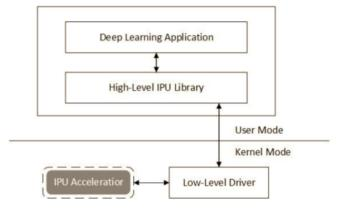
\includegraphics[width=12cm]{IPU.jpg}
\caption{神经网络处理器的架构}
\label{fig:IPU}
\end{figure}

在本文测试过程中,使用的已实现的神经网络处理器架构图如\autoref{fig:IPU}所示。

在用户的应用程序中,为了调用神经网络处理器去准确方便的完成神经网络相关计算,一套稳定可靠的应用程序接口也是不可或缺的。接下来我们将详细介绍神经网络处理器的软件架构。

\section{神经网络处理器的软件架构}
在阐明验证思路之前,我们应首先来熟悉一下神经网络处理器的软件架构, 如\autoref{fig:Software stock}所示,神经网络处理器的软件部分自上而下主要分成如下几个层次:

1.User Program:上层应用,即程序员基于编程框架。定义特定的神经网络结构来实现特定的神经网络功能。

2.Framework:编程框架,相当于连接的桥梁。例如(Caffe、TensorFlow),为用户提供神经网络基本操作,减轻程序员的编程负担,是一种编程工具。

3.runtime library:IPU库是一个屏蔽掉底层硬件,编译器、启动程序的具体信息,对上层编程框架提供神经网络原子(即神经网络的某一层,这是神经网络最基本的组成单元)操作的编程接口的系统软件,它具有内存分配和释放、基本运算、指令生成和数据传输等功能。

IPU库集成封装了神经网络基本的运算操作,如Conv(卷积)、Pooling(池化)、Active(激活函数)、BatchNorm(批规范化)、FullyConnected(全连接)等等常见操作,还有更详细矩阵的数学运算如乘法、加法、减法、缩放等等,这样可以直接调用IPU 的接口,就能直接实现神经网络,同时将优化IPU 的工作封装在IPU 库这一个层次中,而不用直接向应用程序展露。

4.driver、compile:编译器,将上层的库传来的指令描述符按照神经网络处理器的指令集翻译成能接受的机器指令。
驱动:对上层库提供调用底层硬件最基本的操作支持,例如读取数据、启动关闭、读取寄存器等。

5.hardware 硬件:即神经网络处理器(DaDianNao)

\begin{figure}[!htbp]
\centering
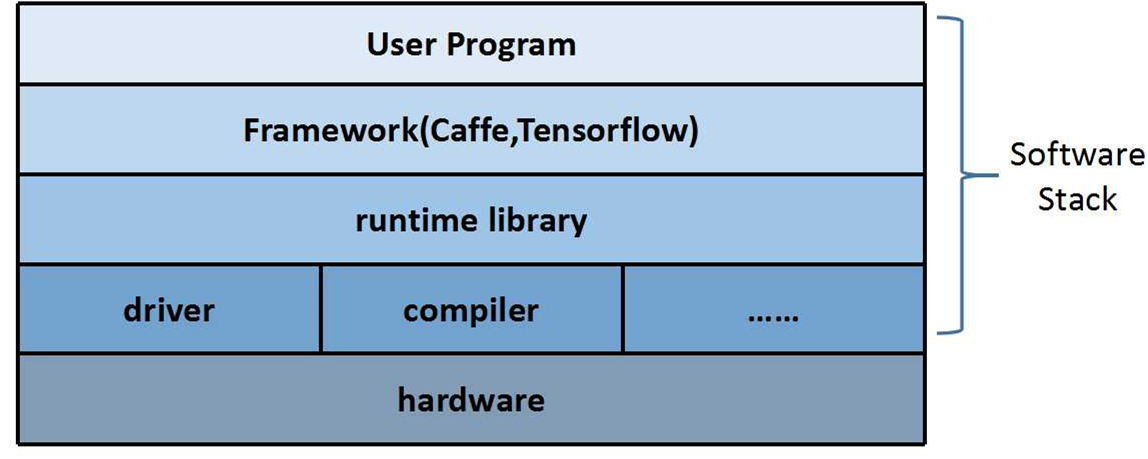
\includegraphics[width=12cm]{Software_stock.jpg}
\caption{神经网络处理器的软件架构}
\label{fig:Software stock}
\end{figure}

\section{测试流程}
在还没有神经网络处理器测试框架的时候,我们曾采取随机生成单个指令的方式来进行验证。然而,由于神经网络处理器指令粒度较大,随机指令无法覆盖到实际使用需求的指令序列,所以需要实际的使用者,也就是编译器生成的指令来做二次审查。这实际上也对应了传统软件测试方法中基于模型测试的思想。

在我们的测试过程中,需要对变量进行控制,由于我们需要测试的是神经网络处理器的编译器,因此主要关注的是库(runtime library)以及编译器(compiler)的正确性。

对于神经网络处理器编译器的验证流程,可以概括为如下几个步骤,首先,生成包含有网络参数与结构信息的配置文件prototxt 。接着,根据prototxt调用caffe提供的接口生成具有训练参数的神经网络模型caffe\underline{ }modrel,然后调用caffe框架,经过一系列的内存分配,指令生成的操作后,调用库的接口,获得神经网络处理器结果,将这个结果caffe中生成的cpu结果进行比对,以达到验证目的。

接下来将详细论述流程的步骤。
\subsection{protext的生成}
要运行caffe,首先需要先创建一个模型(model),caffe里自带了不少常用的神经网络模型,而一个模型由多个层(layer)构成,每一个层又包含多个参数,每一个层的参数都定义在caffe.proto这个文件内。因此,想要生成一个可以用于测试的模型,我们首先得生成一个符合结构要求并含有参数定义的prototxt。

我们自己编写了一套随机网络生成器,通过这个随机网络生成器,我们可以根据用户的需求,生成结构随机,参数随机且具有正确合理的连接方式的神经网络。同时,这个生成器也可以根据用户需求,生成包含有指定层序列、甚至是结构固定的网络,同时,我们也搭建了一个数据库,分三个层次将一些网络的样例加入数据库中。关于随机网络生成器的细节将在第三章详细概述。

\subsection{caffe\underline{ }model的创建}
在得到了包含有网络结构及参数的配置文件prototxt后,我们调用caffe提供的caffe\underline{ }param接口(caffe\underline{ }param是caffe提供的一个记录网络结构与权值并能直接生成caffe\underline{ }model的类),以此初始化一个Net类,在Net中我们将权值初始化,再赋以随机权值传回param类中,而后net\underline{ }param便可以直接将网络结构以及权值写入caffe\underline{ }model中,我们就生成一个具有随机权值的真实网络。

我们先用caffe调用cpu计算数据通过这个网络的结果,而后再调用我们的神经网络处理器。

\subsection{caffe重载}
caffe是一个快速的深度学习框架,现在只能调用cpu与gpu进行计算。因此,为了让caffe能够调用神经网络处理器进行运算,我们对caffe进行了移植,在框架下加入对神经网络处理器硬件的支持。把原来的cpu操作,重载成为神经网络处理器的指令,成为库能接受的操作和运算。

从实现上来看,即将操作的xxx\underline{ }Forward\underline{ }cpu改写为支持神经网络处理器运算的xxx\underline{ }Forward\underline{ }ipu。同时,我们也在内存调度与空间管理等细节上进行了完善,使得caffe可以支持神经网络处理器的运算。

\subsection{caffe调用库的过程}
\begin{figure}[!htbp]
\centering
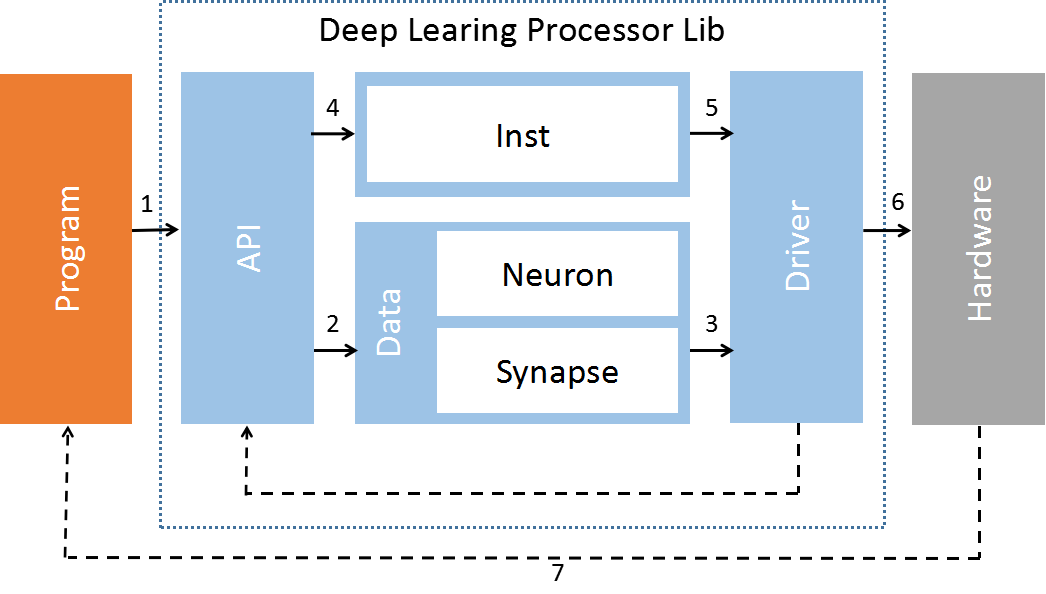
\includegraphics[width=12cm]{DLP1.png}
\caption{库的执行模型}
\label{fig:DLP model}
\end{figure}
caffe运行神经网络处理器的流程如\autoref{fig:DLP model}所示,库的调用大致分为以下流程:

1.初始化神经网络处理器的库

2.声明和设置描述符(tensor描述符,算法描述符,操作描述符)

3.准备数据(nalloc CPU数据和神经网络处理器数据,CPU到神经网络处理器的数据拷贝)

4.IPU运算(xxx\underline{ }Forward函数调用)

5.读取结果

至此,我们已经得到了神经网络处理器结果,将这个结果caffe中生成的cpu结果进行比对,便可以达到验证目的。
\section{测验工作的进程}
对于随机网络生成器来说,现在已经能支持包括卷积,池化,激励等层在内的18种层类型的生成。依靠神经网络处理器测验框架,我们基本完成了库的测试工作,保证了寒武纪系列神经网络处理器编译器的的正确性及可靠性。
\section{本节总结}
本节首先先从神经网络处理器的整体构架说起,而后详细的介绍了神经网络处理器的软件构架并着重点出了我们验证的主要目标。接着,从prototxt的生成到caffemodel的建立,再到caffe的的重载直到最后指令的调用,层层深入,详细介绍了神经网络处理器编译器的验证流程,并简要介绍了使用该测验框架后,测验工作的进程。
  \chapter{随机网络生成器的设计及实现}
要运行Caffe,首先需要先创建一个模型(model),Caffe里自带了不少常用的神经网络模型,而一个模型由多个层(layer)构成,每一个层又包含多个参数,每一个层的参数都定义在caffe.proto这个文件内。因此,想要生成一个可以用于验证的模型,我们必须首先生成一个符合结构要求并含有参数定义的prototxt。
\section{随机网络生成器的设计}
\subsection{prototxt的概述}
prototxt是配置文件,是Caffe中用于描述网络参数以及网络结构的文件。这个文件里不包含对网络训练的权值,相当于一个网络构架。著名的AlexNet网络的prototxt的前四层以及其可视化如\autoref{fig:AlexNet}所示。因此,为了得到一个完整的随机网络,我们应该考虑先生成一个prototxt文件。

\begin{figure}[!htbp]
\centering 
\subfloat[AlexNet网络的prototxt]{
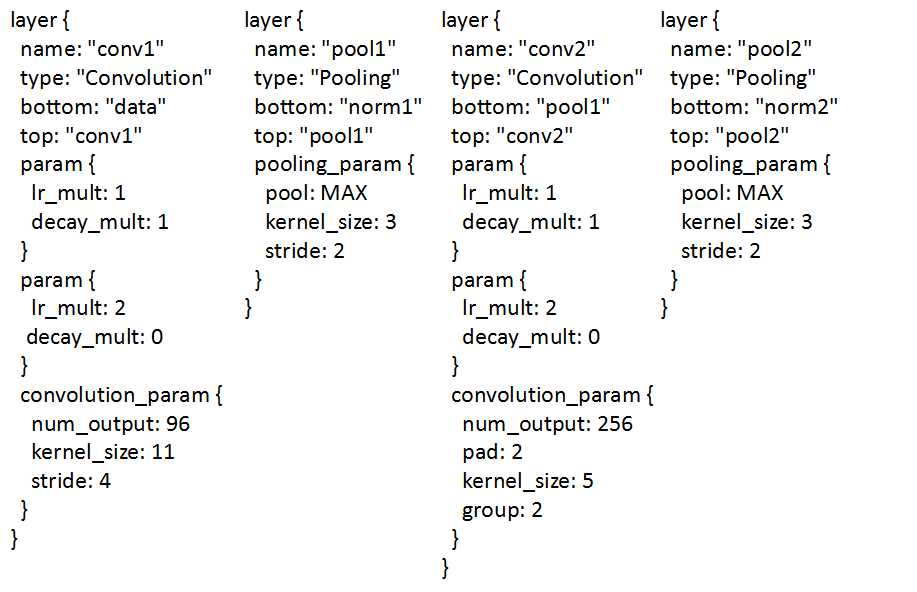
\includegraphics[width=12cm]{Alexnet2.jpg}}
\\
\subfloat[AlexNet网络的可视化]{
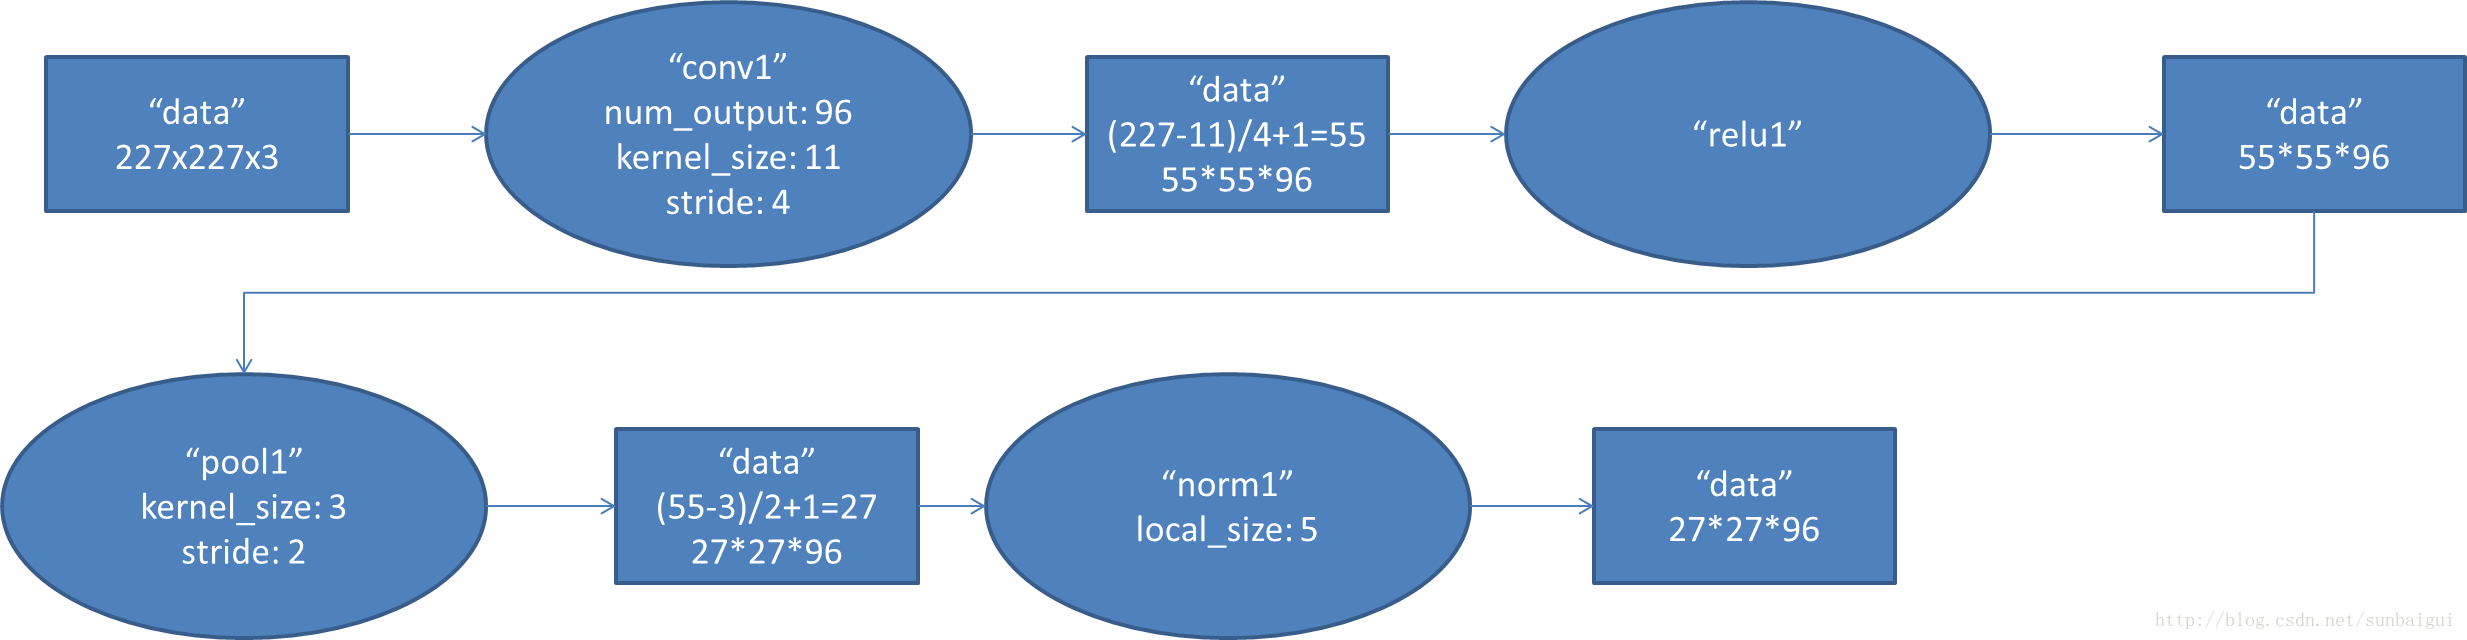
\includegraphics[width=12cm]{Alex1.png}}
\caption{AlexNet网络图}
\label{fig:AlexNet}
\end{figure}

\subsection{随机网络生成器的数据结构}
在我们神经网络生成器当中,有三个主要的数据结构,其一是用于描述网络中最基本粒子“层”的数据结构layer,另一个则是用于描述数据在层之间传递方法的数据结构blob\underline{ }shape。第三个则是用于读取,判断用户对网络结构需求的数据结构struct\underline{ }limit。

下面,我们分别介绍这三个数据结构。
首先,对于blob\underline{ }shape,这是一个一个密集的n维(n $\leq$ 4)阵列,在神经网络中,这代表神经元和偏置(bias)。

在Caffe中也拥有类似的数据结构Blob,用于封装了并在层与层之间传递运行时的信息,提供了CPU和GPU的同步。从数学上来说,Blob就是一个N维数组,是Caffe中的数据操作基本单位,就像matlab中以矩阵为基本操作对象一样。只是矩阵是二维的,而Blob是N维的。N可以是2,3,4等等。对于图片数据来说,Blob可以表示为(N$\times$C$\times$H$\times$W)这样一个4维数组。其中N表示图片的数量,C表示图片的通道数,H和W分别表示图片的高度和宽度。当然,除了图片数据,Blob也可以用于非图片数据。比如传统的多层感知机,就是比较简单的全连接网络,用2维的Blob,调用innerProduct层来计算即可。

而为了与Caffe提供的接口相对应,也为了保证生成网络连接方式的合理性,我们的blob\underline{ }shape也拥有和Caffe中Blob类的类似结构。在我们随机网络生成器中,网络内层与层之间的数据,是用blob\underline{ }shape来表示和运算。它的维度会根据网络参数与结构的类型不同而不同。例如,卷积操作取一个四维的blob\underline{ }shape进行输入,而输出一个四维的blob\underline{ }shape,而全连接操作则取一个四维blob\underline{ }shape进行输入,输出一个二维blob\underline{ }shape。

\begin{figure}[!htbp]
\centering
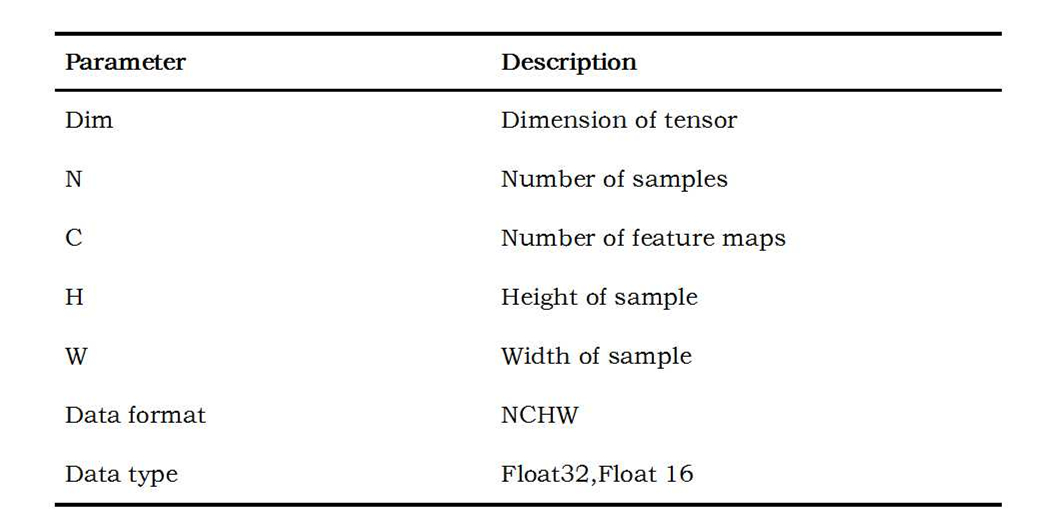
\includegraphics[width=12cm]{Tensor_Structure.jpg}
\caption{blob shape的参数}
\label{fig:Tensor_Structure}
\end{figure}

blob\underline{ }shape描述的属性和参数如\autoref{fig:Tensor_Structure}所示,\emph{N,C,H,W}表示四个维度的大小,其中\emph{N}表示样本数,\emph{C}表示特征映射的数量,也就是图片中通道数,而\emph{H,W}分别表示特征映射的高与宽,每一个数据的数据类型是一个枚举类型变量,用于表示张量的数据格式,这些字母的顺序代表了的blob\underline{ }shape数据排列。

值得注意的是,和Caffe中的Blob相比,我们的blob\underline{ }shape还有一个参数(Dim)用于描述blob\underline{ }shape的维度。对于维度小于4的blob\underline{ }shape,我们也可以用相同的格式来表示。例如,一个二维的blob\underline{ }shape,我们将其H与W设为1,而依靠Dim参数区分H与W都为1的四维blob\underline{ }shape,这样的好处是,我们可以保证数据的传递的有效性,同时也保证了所有的blob\underline{ }shape在网络的传递过程中计算形式上都具有相同的维度,而(Dim)这一参数可以让我们有效地分辨出该数据的实际数值,有效避免了误差。

\begin{figure}[!htbp]
\centering
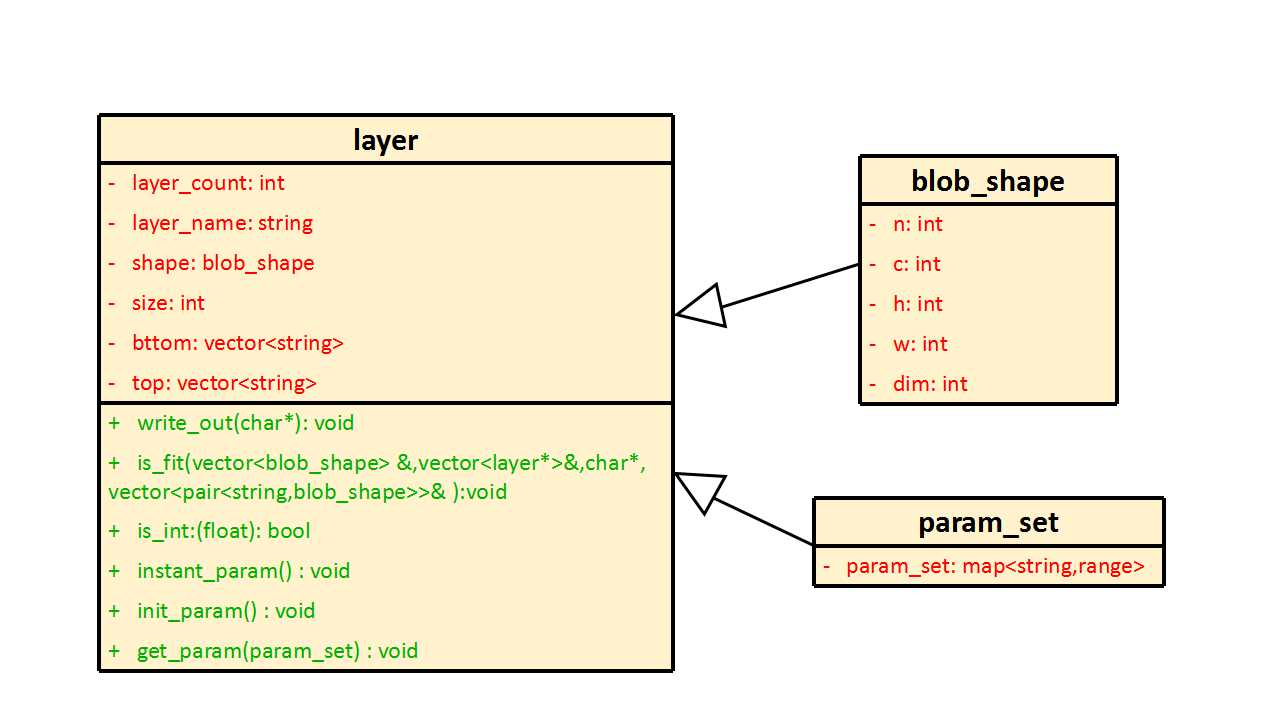
\includegraphics[width=12cm]{layer_blobshape.jpg}
\caption{layer与blobshape的类图}
\label{fig:layer_blobshape}
\end{figure}

对于另一个主要的数据结构——层(layer)来说,神经网络的层是一个独特的概念,这不但代表了一个操作,同时也包含了这个操作的参数,是网络模型的组成要素和基本单位。在Caffe中,proto.prototxt文件记录了每个层的参数种类,但Caffe中layer类用作层与层的运算与数据的传递,而非网络的生成。于是,在我们的随机网络生成器中,层(layer)被声明为一种新的类。这个类里面的变量与方法如\autoref{fig:layer_blobshape}所示。

其中write\underline{ }out方法用来打印网络结构,is\underline{ }fit方法则用于判断单个层(操作)所连接的位置。instant方法和get\underline{ }param方法用于初始化参数范围,前者的初始化是根据设计者估计的参数来设置的,而后者的初始化则是由用户设定的,后者的优先级高于前者,最后由instant方法在范围内随机得到参数,随机参数的类型(整数或者浮点数)由is\underline{ }int控制。

\begin{figure}[!htbp]
\centering
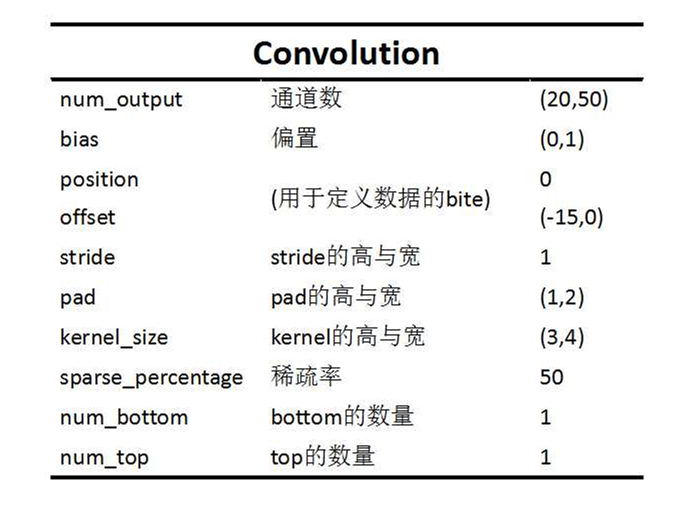
\includegraphics[width=12cm]{conv_param.jpg}
\caption{卷积层的参数类图}
\label{fig:conv_param}
\end{figure}
对神经网络来说,每一个操作(operator)都对应了大量的参数,网络中的layer与每一个operation一一对应。因此也会有众多的参数来描述层的特性。

我们以卷积层(conv\underline{ }layer)为例,说明卷积层内的参数。如\autoref{fig:conv_param}所示,卷积层内有10个参数(后期还可以根据用户的需求进行添加),其中num\underline{ }output,kernel\underline{ }size用于描述核的通道数与长和宽,而pad即stride则用于描述卷积操作中,核(kernel)的具体操作,sparse\underline{ }percentage用于定量描绘稀疏图的概率,这里的每一个参数都在神经网络的卷积操作中有意义,使得程序具有较强的可读性。

第三个数据结构struct\underline{ }limit是用于处理随机神经网络生成器中的结构要求,第一个作用是读取用户单层结构的概率分布,从而按照概率生成所需要的网络,第二个作用则是读取用户输入的串(即给定的layer序列、多层结构)以及串的生成概率,在判断串合法的情况下,生成具有特定连接方式的神经网络。struct\underline{ }limit类里面的变量与方法如\autoref{fig:struct_limit_lei}所示。

其中rule是用于读入用户定义规则的结构体,而snake类则定义了一系列规则,其中add方法用于添加新的规则,而dadj\underline{ }snake方法则用于调整连接规则(例如conv-mlp与mlp-pooling规则可以合成conv-mlp-pooling一条规则)而struct\underline{ }limit继承了两者,用于调配规则,其中series参数用于记录串的形式信息,而rule参数则用来记录用户所提供的生成规则,而check\underline{ }rule方法用于判断合法性。

\begin{figure}[!htbp]
\centering
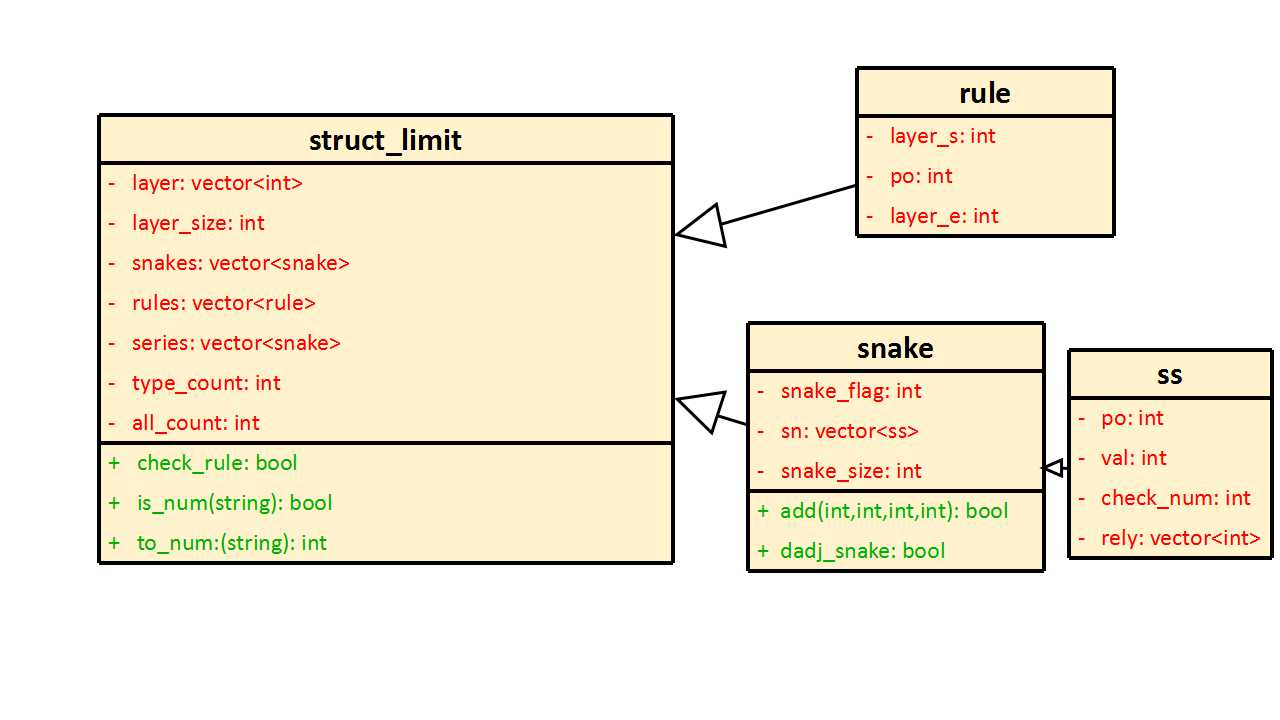
\includegraphics[width=12cm]{struct_limit_lei.jpg}
\caption{struct limit的类图}
\label{fig:struct_limit_lei}
\end{figure}

\subsection{网络的建立}
网络是由层(layer)构成,而blob\underline{ }shape封装了数据从layer一层一层输入再输出。而数据数据能否作为一个层的输入是取决于数据的维度、数值以及层的参数,而数据的输出则在层中根据层的种类与参数进行计算与调配。

卷积层是卷积神经网络(CNN)最重要的一种层的类型,它需要一个四维blob\underline{ }shape作为输出,并输出一个四维blob\underline{ }shape。张量的操作通过层来进行,卷积层的参数类型如\autoref{fig:conv_param}所示,一个blob\underline{ }shape传入卷积层后,N值保持不变,C值被卷基层的number\underline{ }output所取代,而H和W则由\autoref{eq:1.1}与\autoref{eq:1.2}计算:
\begin{equation}\label{eq:1.1}
H=\lceil \frac{H_{i}-K_h+1+2P_{h}}{S_{h}}\rceil
\end{equation}
\begin{equation}\label{eq:1.2}
W=\lceil \frac{W_{i}-K_w+1+2P_{w}}{S_{w}}\rceil
\end{equation}
其中$H_{i}$和$W_{i}$代表输入张量的H和W,$K_h$与$K_w$则代表了kernel的长和宽,而$P_h$,$P_w$则代表了pad的长和宽,这些都能在层的参数中得到,之后将得到的新的张量存储在shape中传向网络里更深的位置(层)内。

在blob\underline{ }shape的传入与输出过程中,is\underline{ }fit函数能控制输入的合法性,例如对于平常的卷积层,我们需要保证输入的blob\underline{ }shape是四维的,同时,输出的blob\underline{ }shape里,每一个成员变量都需要大于0,即还应该满足\autoref{eq:1.3}与\autoref{eq:1.4}:
\begin{equation}\label{eq:1.3}
\lceil H_{i}-K_h+1+2P_{h}\rceil >0
\end{equation}
\begin{equation}\label{eq:1.4}
\lceil W_{i}-K_w+1+2P_{w}\rceil >0
\end{equation}
对于一些操作复杂的层来说is\underline{ }fit函数还取到了生成补充层的作用,例如eltwise层需要输入多个blob\underline{ }shape,同时保证输入blob\underline{ }shape的四个维度都相等,而lstm\underline{ }unit层则既输入多个blob\underline{ }shape,同时也输出多个blob\underline{ }shape,进一步的,我们还可以根据库的要求、乃至硬件的要求调整is\underline{ }fit函数,使得该程序具有很好的可扩展性。
\section{随机网络生成器的实现}
\subsection{随机网络生成器的运行}
主函数首先读取struct\underline{ }limit以及param\underline{ }limit两个文件,前者用于描述网络的结构分布,即网络的深度以及每一类型的层在本次随机网络生成中所占有的比例,后者则用于描述不同层中参数的限制。这些结构分布与参数限制都根据用户的验证需求自行限制。另外,除了每次进行单个层的生成与连接外,还可以把多个层构成串一并连接并生成。例如,我们可以要求每一个卷积层(convolution)后面,连接的都是一个全连接层(mlp),这样子尽可能满足了用户的验证需求,也给程序的维护带来了便利。

\begin{figure}[!htbp]
\centering 
\subfloat[网络结构限制]{
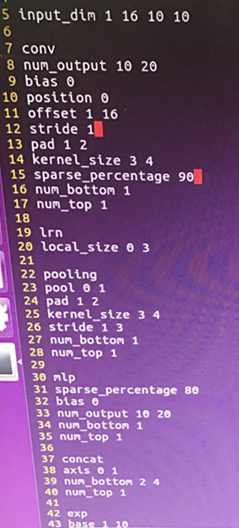
\includegraphics[width=4.5cm]{param_limit.jpg}}
\subfloat[网络参数限制]{
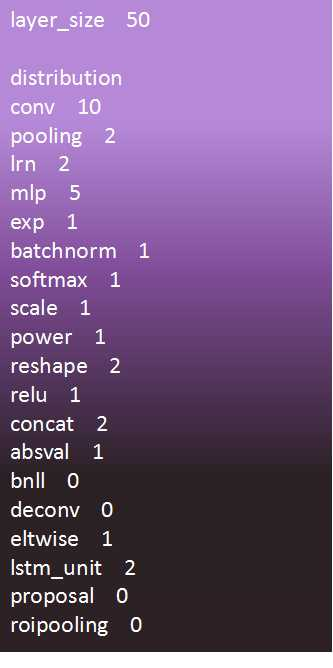
\includegraphics[width=4.5cm]{struct_limit.jpg}}
\caption{proto的运行}
\label{fig:limit}
\end{figure}
\section{caffe\underline{ }model的生成}

在读取参数后,主函数根据用户的需求按规则生成我们所需要的网络,并调用write\underline{ }out方法从而打印生成具有网络信息的prototxt文件。我们现在得到了网络信息,然而这个网络还是一个“空架子”,我们接下来先根据每一个层的连接方式,为网络补充上权值,我们写了一个create\underline{ }model函数,主要的作用就是调用Caffe提供的caffe\underline{ }param接口(caffe\underline{ }param是caffe提供的一个记录网络结构与权值并能直接生成caffe\underline{ }model的类),初始化一个Net类,在Net中我们将权值初始化,再赋值传回param类中,而后net\underline{ }param可以直接将网络结构以及权值写入caffe\underline{ }model中,至此,我们生成一个具有随机权值的真实网络,简单的说就是我们将一个“空架子”给“填充”了。这样子,便生成了我们所需要的 caffe\underline{ }model。

\subsection{生成已有的常用网络}
在前文中,我们已经介绍了随机网络模型的生成流程,虽然已有的常用网络(例如Lenet,Alex等)是随机网络模型的子集,但常用网络的训练效果已得到同行的验证,因此在我们神经网络处理器测试框架的测试中,具有一定的代表性,同时将已有的常用网络单独测试也可以增强开发者的信心。

对于常用网络,Caffe里面已经给出了现有的prototxt,甚至也有提供已经训练好的caffe\underline{ }model,因此,我们无需再去生成。(事实上,我们的随机网络模型生成器也可以按照给定的串生成常用网络),之后调用Caffe提供的caffe\underline{ }param接口,便可以生成具有随机权值的常用网络模型了。

\subsection{测试框架数据库的建立}
高效的测试需要有数据库来支持。对于神经网络处理器编译器的验证来说,由于bug主要出现在指令集中,由于神经网络处理器的特殊性,即使是同一条指令,不同的参数,指令的生存周期变化很大,且需要访问的存储范围变化也很大,所以我们的数据库里应该记载了完整的神经网络结构。我们的数据库应该由如下几个层次构成:

1.单个层随机参数的指令,因为随着库能支持的网络越来越多,需要验证的网络种类也会越来越复杂,因此,我们需要对网络的最基本构造——层进行单独测试。因此,对于每一种新的层,我们应该把单层的网络加入到库中。

2.已有的常用网络,常用的网络具有代表性,同时验证常用网络也会给予开发者信心,因此我们会收集其他同行使用过的网络,在库支持的前提下,对其进行验证。

3.之前出过错的网络结构。由于神经网络结构的复杂性,因此修正了一个错误有可能会导致其他错误,将这些corner case 收集,在每一次改良调试库之后,优先对这些网络结构进行测试,可以较容易的发现错误。这里也运用到了前文中介绍的回归测试的软件验证思想。
\section{本节总结}
第四章介绍了神经网络处理器编译器测试框架中最重要的随机网络生成器的实现。吸取了编程框架Caffe中数据结构的优点并对其结构进行改良,将层的连接方式以及网络的构建融入网络生成器的创建当中,并实现了一系列方法用于满足用户对结构以及参数的要求,最后,建立了一个数据库用于保证测试的高效性,同时阐述了数据库的设计思想。
  %\chapter{验证框架能的支持及改进}

\section{如今能支持的需求}

\section{还需要改进的地方}
  \chapter{展望与总结}
\section{工作总结}
论文从深度学习入手,介绍了现有的CPU、GPU 在面对大规模的深度学习神经网络应用时的困境,从而引入了专用于深度学习神经网络的神经网络处理器。为了能让用户正确稳定的使用神经网络处理器,神经网络处理器编译器的测试工作是很重要的,同时,由于神经网络处理器内部运算部件和数据存储结构等多方面创新性的不同,一套能用于检测神经网络处理器编译器的测试框架是必要的。

在调研了传统软件以及传统编译器的测试方式后,我们结合传统软件测试的方法和神经网络处理器编译器的独特性质,设计了一套专门用于检测神经网络处理器编译器的测试框架,通过该测试框架,我们提高了测试效率。

最后,我们详细地阐述了测试框架中最重要的一环——随机神经网络生成器,解释了随机网络生成器的功能和实现方法,最后,我们搭建了一个数据库来保证测试工作的高效性并解释了数据库的设计思想。

\section{下一步研究方向}
对于神经网络处理器编译器测试工作来说,我们接下来将继续完善我们的随机网络生成器,增加能支持的操作类型。除外,我们还将继续移植其他主流编程框架、并对新的编译器进行测试。

神经网络处理器编译器的复杂性,决定了我们测试工作的复杂性;而我们测试工作的高效性,则决定了编译器乃至整个神经网络处理器的高效性,为此,我们将会不断努力。
  %自行添加
  %\include{chapter/...}

%%%%%%%%%%%%%%%%%%%%%%%%%%%%%%
%% 附件部分
%%%%%%%%%%%%%%%%%%%%%%%%%%%%%%
\backmatter

  % 参考文献
  % 使用 BibTeX
  % 选择参考文献的排版格式。注意ustcbib这个格式不保证完全符合要求,请自行决定是否使用
  \bibliographystyle{ustcbib}%{GBT7714-2005NLang-UTF8}
  \bibliography{bib/tex}
  %\nocite{*} % for every item
  % 不使用 BibTeX
  % %\renewcommand{\baselinestretch}{0.5}
\begin{thebibliography}{10}

\bibitem{deng:01a}
{邓建松,~彭冉冉,~陈长松邓建松,~彭冉冉,~陈长松邓建松,~彭冉冉,~陈长松邓建松,~彭冉冉,~陈长松邓建松,~彭冉冉,~陈长松邓建松,~彭冉冉,~陈长松邓建松,~彭冉冉,~陈长松邓建松,~彭冉冉,~陈长松邓建松,~彭冉冉,~陈长松邓建松,~彭冉冉,~陈长松邓建松,~彭冉冉,~陈长松}.
\newblock {\em \LaTeXe{}~科技排版指南}.
\newblock 科学出版社,~书号:~7-03-009239-2/TP.1516, 北京, 2001.

\bibitem{wang:00a}
王磊.
\newblock {\em \LaTeXe{}~插图指南}.
\newblock 2000.

\bibitem{zhang:03a}
张林波.
\newblock {\em 关于新版~CCT~的说明}.
\newblock 2003.

\bibitem{lshort-cn}
C\TeX{} 翻译小组.
\newblock {\em lshort~中文版~3.20}.
\newblock 2003.

\bibitem{knuth86e}
Donald~E. Knuth.
\newblock {\em Computer Modern Typefaces}, volume~E of {\em Computers and
  Typesetting}.
\newblock Addison-Wesley, Reading, Massachusetts, 1986.

\bibitem{knuth86d}
Donald~E. Knuth.
\newblock {\em {METAFONT}: The Program}, volume~D of {\em Computers and
  Typesetting}.
\newblock Addison-Wesley, Reading, Massachusetts, 1986.

\bibitem{knuth86c}
Donald~E. Knuth.
\newblock {\em The {METAFONT}book}, volume~C of {\em Computers and
  Typesetting}.
\newblock Addison-Wesley, Reading, Massachusetts, 1986.

\bibitem{knuth86b}
Donald~E. Knuth.
\newblock {\em {TeX}: The Program}, volume~B of {\em Computers and
  Typesetting}.
\newblock Addison-Wesley, Reading, Massachusetts, 1986.

\bibitem{knuth86a}
Donald~E. Knuth.
\newblock {\em The {TeX}book}, volume~A of {\em Computers and Typesetting}.
\newblock Addison-Wesley, Reading, Massachusetts, 1986.

\bibitem{lamport85a}
Leslie Lamport.
\newblock {\em {LaTeX} --- A Document Preparation System: User's Guide and
  Reference Manual}.
\newblock Addison-Wesley, Reading, Massachusetts, 2nd edition, 1985.

\end{thebibliography}


  % 附录,没有请注释掉
  %\begin{appendix}
  %\chapter{中国科学技术大学研究生学位论文撰写规范}
\label{chap:requires}
\section*{以下文字仅作示例,一切以学校规定为准!}
研究生院规定在此下载\url{http://gradschool.ustc.edu.cn/ylb/material/xw/wdxz/1.doc}

研究生学位论文集中反映研究生在研究工作中所取得的成果,代表研究生研究工作的水平,也是申请和授予相应学位的主要依据。为提高研究生学位论文的撰写质量,做到学位论文在内容和格式上的规范化,我们编写了《中国科学技术大学研究生学位论文撰写规范》,供申请学位的研究生参考执行。其中参考文献著录规则我们根据GB/T 7714-2005的标准撰写。硕士和博士学位论文除在研究深度等方面要求不同外,撰写要求基本一致。

\section{内容要求}

\subsection{封面} 
采用研究生院规定的统一封面,封面包含内容如下: 
\subsubsection{密级} 涉密论文必须在论文封面标注密级(内部、秘密、机密),同时注明保密年限。
\subsubsection{论文题目} 应准确概括整个论文的核心内容,简明扼要,最多不超过30字,必要时可以加副标题。
\subsubsection{作者姓名} 英文封面中按英文习惯书写,即名在前。姓名需写全拼。
\subsubsection{学科专业} 写所在专业的全称,不可用简写。
\subsubsection{导师姓名} 一般允许有两名指导教师,主要指导教师姓名写在第一位,后附其职称,次要指导教师排第二位,也需注明职称。
\subsubsection{完成时间} 填写论文打印成文的年月日。

\subsection{中国科学技术大学学位论文原创性和授权使用声明}
本部分内容使用统一的模版,具体内容见格式范例,提交时作者须亲笔签名。

\subsection{摘要和关键词}
\subsubsection{中文摘要}
摘要是论文内容的总结概括,应简要说明论文的研究目的、基本研究内容、研究方法、创新性成果及其理论与实际意义,突出论文的创新之处。不宜使用公式、图表,不标注引用文献。 
\subsubsection{中文关键词} 
关键词是为了文献标引工作从论文中选取出来用以表示全文主题内容信息的单词和术语,一般3--8个词,要求能够准确概括论文的核心内容。
\subsubsection{英文摘要与关键词}
以中文书写的论文,内容与中文摘要和关键词完全一致,其他语种书写的论文以简略为原则,不需要相同。

\subsection{目录}
目录页由论文的章、条、附录等序号、名称和页码组成。论文中如图表较多,可以分别列出清单置于目次页之后。图的清单应有序号、图题和页码。表的清单应有序号、表题和页码。

\subsection{符号说明}
如果论文中使用了大量的物理量符号、标志、缩略词、专门计量单位、自定义名词和术语等,应编写成注释说明汇集表。若上述符号等使用数量不多,可以不设此部分,但必须在论文中出现时加以说明。

\subsection{正文}
正文是学位论文的主体,包括绪论、论文主体及结论等部分。
\subsubsection{绪论}
内容应包括:选题的背景和意义,文献综述及研究现状,研究内容与预期结果,研究方法和实验设计,论文结构安排等。要求实事求是,不夸大、缩小前人的工作和自己的工作,言简意赅,突出重点,不与摘要雷同。
\subsubsection{论文主体}
论文主体是正文的核心部分,占主要篇幅,它是将学习、研究和调查过程中筛选、观察和测试所获得的材料,经过加工整理和分析研究,由材料而形成论点。由于各学科及具体选题的差异,此部分不作统一规定。但总体内容必须实事求是,客观真切,准确完备,合乎逻辑,层次分明,简练可读。
\subsubsection{结论}
结论是对整个论文主要成果的总结,应明确、精炼、完整、准确。其中应明确指出本研究的创新点,对论文的学术价值和应用价值等加以预测和评价,说明研究中尚难解决的问题并提出今后进一步在本研究方向进行研究工作的设想或建议。

\subsection{参考文献}
本着以严谨求实的科学态度撰写论文,凡学位论文中有引用或参考、借用他人成果之处,均应详细列出所引文献的名称、作者、发表刊物、发表时间、卷号、页码等,严禁抄袭剽窃。  
\subsection{附录}
主要列入正文内过分冗长的公式推导,供查读方便所需的辅助性数学工具或表格,重复性数据图表,论文使用的缩写,程序全文及说明等。

\subsection{致谢}
对给予各类资助、指导和协助完成研究工作以及提供各种对论文工作有利条件的单位及个人表示感谢。致谢应实事求是,切忌浮夸与庸俗之词。

\subsection{在读期间发表的学术论文与取得的其他研究成果}
按学术论文发表的时间顺序,列齐本人在攻读学位期间发表或已录用的学术论文清单(发表刊物名称、卷册号、页码、年月及论文署名、作者排序)。其他研究成果可以是申请的专利、获得的奖项及完成的项目等。
 
\section{书写规定}

\subsection{论文的字数要求}
硕士学位论文要求不少于3万字,博士学位论文要求不少于5万字。

\subsection{文字、标点符号和数字}
除留学生和外语专业研究生外,学位论文一律用汉字书写。除非特殊需要,不得使用已废除的繁体字、异体字等不规范汉字。标点符号的用法以GB/T 15834—1995《标点符号用法》为准。数字用法以GB/T 15835—1995《出版物上数字用法的规定》为准。

留学生的学位论文所采用语种可以和导师商定,但论文封面须用中文。

\subsection{封面与扉页}
\subsubsection{秘级} 封面的秘级可以标注为内部、秘密和机密,各密级的保密时限分别为小于等于5年、小于等于10年和小于等于20年,非保密论文不标注密级。
\subsubsection{题目} 题目中避免使用缩略词、首字母缩写字、字符、代号和公式等。
\subsubsection{日期} 封面的日期用汉字书写。
\subsubsection{扉页} 扉页的内容与封面一致。扉页后,需给出英文的封面。其他语种书写的论文还需在英文封面后附上正文所用语种书写的封面。

\subsection{目录}
目录应包括论文的全部内容,包括中英文摘要和附录等,正文章节题名要求编到第3级标题,即×.×.×。一级标题顶格书写,二级标题缩进一个汉字符位置,三级标题缩进两个汉字符位置。

\subsection{摘要与关键词}
\subsubsection{摘要}
摘要分中文和英文两种,中文在前,英文在后。标题摘要二字中间空一格。摘要的字数,硕士学位论文建议1000字以内,博士学位论文建议3000字以内。留学生用其他语种撰写学位论文时,中文摘要应不少于6000汉字。摘要中不得出现图片、图表、表格或其他插图材料。英文摘要与中文摘要应完全一致。
\subsubsection{关键词}
关键词以显著的字符另起一行并隔行排列于摘要下方,左顶格。中文关键词间空一格,英文关键词间用逗号隔开。

\subsection{论文正文}
\subsubsection{章节及各章标题}
论文正文分章节撰写,每章应另起一页。

各章标题字数一般应在15字以内,不使用标点符号。标题中尽量不采用英文缩写词,对必须采用者,应使用本行业的通用缩写词。
\subsubsection{序号}
\paragraph{标题序号}
论文标题分层设序。层次以少为宜,根据实际需要选择。各层次标题一律用阿拉伯数字连续编号;不同层次的数字之间用小圆点“.”相隔,末位数字后面不加点号,如“1”,“1.1”,“1.1.1”等;各层次的序号均左起顶格排,后空1个字距接排标题。例如:

第1章 ××××(大标题) 

1.1 ××××(一级节标题)

1.1.1 ××××(二级节标题)

1.1.1.1 ××××(根据需要,也可设三级节标题)

第2章 ××××(大标题)

2.1 ××××(一级节标题)

2.1.1 ××××(二级节标题)

\paragraph{图表等编号} 
论文中的图、表、附注、公式、算式等,一律用阿拉伯数字分章依序连续编码。其标注形式应便于互相区别,如:图 l.1(第1章第一个图)、图2.2(第二章第二个图);表3.2(第三章第二个表)等。
\paragraph{页码}
页码从绪论开始按阿拉伯数字(1,2,3……)连续编排,此前的部分(中英文摘要、目录等)用大写罗马数字(I,II,III…)单独编排,页码位置居于页脚居中。封面、扉页、创新性声明等不编页码。
\subsubsection{页眉}
页眉从中文摘要开始,内容与该部分的一级标题相同,奇偶页相同,各部分的首页也需有页眉。
\subsubsection{名词和术语}
科技名词术语及设备、元件的名称,应采用国家标准或部颁标准中规定的术语或名称。标准中未规定的术语要采用行业通用术语或名称。全文名词术语必须统一。一些特殊名词或新名词应在适当位置加以说明或注解。

采用英语缩写词时,除本行业广泛应用的通用缩写词外,文中第一次出现的缩写词应该用括号注明英文原词。
\subsubsection{量和单位}
量和单位要严格执行GB 3100~3102-93(国家技术监督局1993-12-27发布,1994-07-01实施)有关量和单位的规定。

量的符号一般为单个拉丁字母或希腊字母,并一律采用斜体(pH例外)。为区别不同情况,可在量符号上附加角标。 

在表达量值时,在公式、图、表和文字叙述中,一律使用单位的国际符号,且无例外地用正体。单位符号与数值间要留适当间隙。具体可参见下列表达式3.1。

\subsubsection{图和表}
\paragraph{图}
图应具有“自明性”,即只看图、图题和图例,不阅读正文,就可理解图意。每一图应有简短确切的题名,连同图号置于图下。

图的位置在相关说明文字之后,随文排。坐标比例不宜过大,同一图上不同曲线的点要分别用不同形状的标识符标出。图中的术语、符号、单位等应与正文表述中所用一致。

图题应简明。图号和图题间空1个字符位置,居中排于图的下方。

必要时,应将图上的符号、标记、代码,以及实验条件等,用最简练的文字,横排于图题下方,作为图例说明(图注)。

\paragraph{表}
表的位置也在相应说明文字之后,随文排。表中参数应标明量和单位的符号。表应有自明性。每一表应有简短确切的题名,连同表号置于表上,表号与表题间空一个字符位置。表号用阿拉伯数字分章编号,如第3章第2个表的表号表示为“表3.2”。

表格太大需要转页时,需要在续表上方注明“续表”,表头也应重复排出。

必要时应将表中的符号、标记、代码,以及需要说明事项,以最简练的文字,横排于表题下,作为表注。相关要求同于图注。

\subsubsection{表达式}
表达式主要指数字表达式,也包括文字表达式。表达式需另行起排,原则上应居中,用阿拉伯数字分章编号。序号加圆括号,右顶格排。例如,第3章第1个表达式:

较长的式如必须转行,只能在+,-,×,÷,<,>处转行,序号编于最后一行的最右边。

\subsection{参考文献}
参考文献参照GB/T 7714-2005《文后参考文献著录规则》执行。推荐使用著者-出版年制,即在正文引用文献处标注著者姓名与出版年份,在文后的参考文献表中标注参考文献的详细信息。
\subsubsection{著者-出版年制在正文中的标注方式}

正文中的标注方式分两种:其一,正文里已出现著作者姓名的,在其后用圆括号附上出版年份即可;其二,正文里仅提及有关的资料内容而未提到著作者,则在相应文句处用圆括号标注著作者姓名和出版年份,两者之间加逗号。

例如:

Park et al(1995)根据Laurentia西缘放射状基性岩墙的研究以及与地幔柱有关的澳大利亚Gairdner岩墙群的研究,首次提出约780Ma地幔柱导致Rodinia超大陆的裂解。

其中关于成冰系顶底界时限和冰川活动年龄、超大陆裂解的起始时间和持续时间……是当前中国地球科学界十分活跃并得到迅速发展的研究领域(王平,2003)。

引用同一著者在同一年份出版的多篇文献时,在出版年份之后用英文小写字母a、b、c……区别。如:(王平,2005a);(王平,2005b)

多处引用同一著者的同一文献时,在“()”外以角标的形式著录引文页码。引用有两个以上同姓的著者的外文文献时,则著者要加名字的缩写,但不必加缩写点。

引用多位著者的文献时,对欧美著者只需标注第一个著者的姓,其后附“et al”,仅两位作者的也可全部注出,中间用“and”;对中国著者应该标注第一著者的姓名,其后附“等”字,姓名与“等”字之间留1个空格。例如:……(王平 等,2005) ……。

同一处引用多篇文献时,按出版年份由近及远依次标注,中间用逗号分开。

\subsubsection{著者-出版年制参考文献表的编排}
 参考文献表加居中标题——“参考文献”,并列入全书目录。

凡正文里括注了著者姓名和年份的,其文献都必须列入参考文献表。

参考文献表中的条目(不排序号),先按语种分类排列,语种顺序是:中文、日文、英文、俄文、其他文种。然后,中文和日文按第一著者的姓氏笔画排序,中文也可按汉语拼音字母顺序排列,西文和俄文按第一著者姓氏首字母顺序排列。

在参考文献中,当一个著者有多篇文献并为第一著作者时,他单独署名的文献排在前面(并按出版年份的先后排列),接着排他与其他人合写的文献。

著录项目与GB/T 7714-2005《文后参考文献著录规则》中规定的顺序编码制基本相同,不同的仅为出版年份排于编著者之后。
\subsubsection{参考文献标注的注意事项}
编著者姓名,一律姓在前、名字在后。西文和俄文的姓全部著录,名字可用大写首字母(不加缩写点);如果姓和名的首字母相同,便要用全名。

以机构和团体署名的文献,此机构或团体可作为编著者,但要用全称,而不用简称或缩写。

编著者不明的文献,编著者一项应注明“佚名”,或用其他与之相应的词。 

编著者为3人以下时全部著录,用逗号分隔,3人以上可只著录前3人,后加“,等”,外文用“,et al”,“et al”不必用斜体。

外文文献大写字母的使用要符合文种本身的习惯用法。

外文期刊刊名可列出全名,也可列惯用缩写刊名(缩写点可加,也可不加,但全文要统一)。只有一个词的刊名不能缩写。期刊名排正体。

期刊只列出卷号,不必标“卷”或“Vol”等;如果是分卷图书,则应加“卷”或“册”或“Vol”或其他语种相应的词(外文缩写词不加缩写点,首字母大小写应全文统一)。

参考文献的版次、卷、期、页码等数字一律用阿拉伯数字表示。版次中中文版次著录为“第2版”、“第3版”……(第1版不必列出),西文文献的版次著录为“2nd ed”、“3rd ed”或其他语种相应的词 。

出版年采用公元纪年,并用阿拉伯数字著录。如有其他纪年形式时,将原有的纪年形式置于“( )”内。

如:1947(民国三十六年)

日文文献中的汉字要用日文汉字。

参考文献中使用的标点符号:

,用于多著者姓名之间,出版者和年或卷(期)之间,期刊名和年或卷之间,“等”或“译”字、专利号等之前。

:用于副题名之前、出版地之后,或引文页码、析出文献页码、专利国别前。

()用于期号、报纸的版次、电子文献更新或修改日期以及非公元纪年。

[] 用于序号、文献类型、电子文献的引用日期以及自拟的的信息。

∥用于专著中的析出文献的出处项前。

- 用于起讫序号和起讫页码间。

. 用于其余各项目之后。

\subsubsection{顺序编码制的著录规则}
参考文献如果按照顺序编码制著录,可参照GB/T 7714-2005《文后参考文献著录规则》执行。


\section{排版和印刷要求}略

\chapter{关于规范本科毕业论文(设计)格式和统一封面的通知}
\section*{以下文字仅作示例,一切以学校规定为准!}
教务处规定在此下载\url{http://202.38.70.92/bklw.doc}

\hspace{-2em}各院系:

鉴于目前各院系本科毕业论文(设计)存在着论文格式不够规范、封面不统一的状况,为加强本科毕业论文的管理,提高论文质量,同时规范全校本科毕业论文(设计)格式,现对本科毕业论文格式和统一封面规定如下:
\begin{enumerate}
\item 本科毕业论文按编排顺序应包括以下内容:封面、扉页、致谢、目录、中文内容摘要、英文内容摘要、正文章节、参考文献或资料注释、附录等。
\item 本科毕业论文的格式要求:
\begin{enumerate}
\item 封面中“论文题目”等内容用四号宋体。
\item 除封面、扉页外,每面上部加页眉,用小5号字标注“中国科学技术大学本科毕业论文”,居中。
\item 从目录页开始在每面底部居中用小五宋体连续编页码。
\item 论文的“致谢”、“目录”等标题用小二号黑体字,居中。
\item 目录一般列三级,后附规范的页号。
\item 正文中的标题分章、节、段三级;章、节标题居中,段标题居左,分别用三号黑体、小三黑体、四号黑体。
\item 具体内容用小四号宋体,每行间距为22磅,科学公式和符号要符合国标,公式要单独占行、居中、行距为单倍行距。
\item 表格、插图全文要分别统一编号或按章编号,标题用小四宋体:(表格标题居表上方,插图标题居图下方),居中。
\item 参考文献的内容包括:序号、作者名、书名或文章名、刊物名或出版社名、
刊物期卷、页和日期,用小四宋体,外文期刊名用白斜体。
\item 附录为:
\begin{enumerate}
\item 重要参考文献中相关内容和章节复印件;
\item 作者或导师所做的与本论文有关的成果复印件。
要求用A4纸复印附于参考文献后。
\end{enumerate}
\end{enumerate}
\item 本科毕业论文(设计)封面学校已统一印制,请到教材科领购。
\item 装订要求:每份论文必须用A4纸打印(复印)、装订成册(教材科可提供复印、装订业务)。另外,校级优秀毕业论文必须提交一份线装毕业论文交档案馆收藏。
\item 具体格式详见附件式样。
\end{enumerate}
\begin{flushright}
中国科技大学教务处

二OO二年三月二十八日
\end{flushright}
附件:本科毕业论文(设计)式样

(略)

  %\end{appendix}

  \makeatletter
  \ifustc@bachelor\relax\else
    % 致谢
	
\begin{thanks}

感谢原本科模板的作者XPS、硕博模板的作者刘青松以及它们的维护者的辛勤工作!

感谢大家对本模板更新工作的支持!

本模板以及本示例文档还存在许多不足之处,欢迎大家测试并及时提供反馈。

\begin{flushright}
ywg@USTC
\end{flushright}


在中国科技大学完成本科和硕博连读学业的九年里,我所从事的学习和研究工作,都是在导师以及系里其他老师和同学的指导和帮助下进行的。在完成论文之际,请容许我对他们表达诚挚的谢意。

首先感谢导师XXX教授和XXX副教授多年的指导和教诲,是他们把我带到了计算机视觉的研究领域。X老师严谨的研究态度及忘我的工作精神,X老师认真细致的治学态度及宽广的胸怀,都将使我受益终身。

感谢班主任XXX老师和XX老师多年的关怀。感谢XXX、XX、XX等老师,他们本科及研究生阶段的指导给我研究生阶段的研究工作打下了基础。

感谢XX、XXX、XXX、XX、XXX、XXX、XXX、XX等师兄师姐们的指点和照顾;感谢XXX、XX、XXX等几位同班同学,与你们的讨论使我受益良多;感谢XXX、XX、XXX、XX、XXX等师弟师妹,我们在XXX实验室共同学习共同生活,一起走过了这段愉快而难忘的岁月。

感谢科大,感谢一路走过来的兄弟姐妹们,在最宝贵年华里,是你们伴随着我的成长。

最后,感谢我家人一贯的鼓励和支持,你们是我追求学业的坚强后盾。

\vskip 18pt

\begin{flushright}

~~~~赵钱孙~~~~

\today

\end{flushright}

\end{thanks}
%硕博致谢部分
    % 发表文章目录
    
\chapter{在读期间发表的学术论文与取得的研究成果}

\noindent\textbf{研究工作:}

\begin{enumerate}

\item A A A A A A A A A
\item A A A A A A A A A
\item A A A A A A A A A
\item A A A A A A A A A

\end{enumerate}


\noindent\textbf{已发表论文:}

\begin{enumerate}

\item A A A A A A A A A 
\item A A A A A A A A A
\item A A A A A A A A A
\item A A A A A A A A A
\item A A A A A A A A A
\item A A A A A A A A A
\item A A A A A A A A A
\item A A A A A A A A A

\end{enumerate}

\vskip 1cm

\noindent\textbf{待发表论文:}

\begin{enumerate}

\item A A A A A A A A A

\end{enumerate} 
  \fi
  \makeatother

\end{document}
